\chapter{Other Supernova Remnants}\label{chp:chp6}

%\begin{flushright}
%  {\em QUOTE GOES HERE }\\
%
%\ \
%
%\normalsize
%{AUTHOR}  
%\end{flushright}


\noindent{FIRST PARAGRAPH}

\section{SN 1980K}

\begin{figure}
\centering
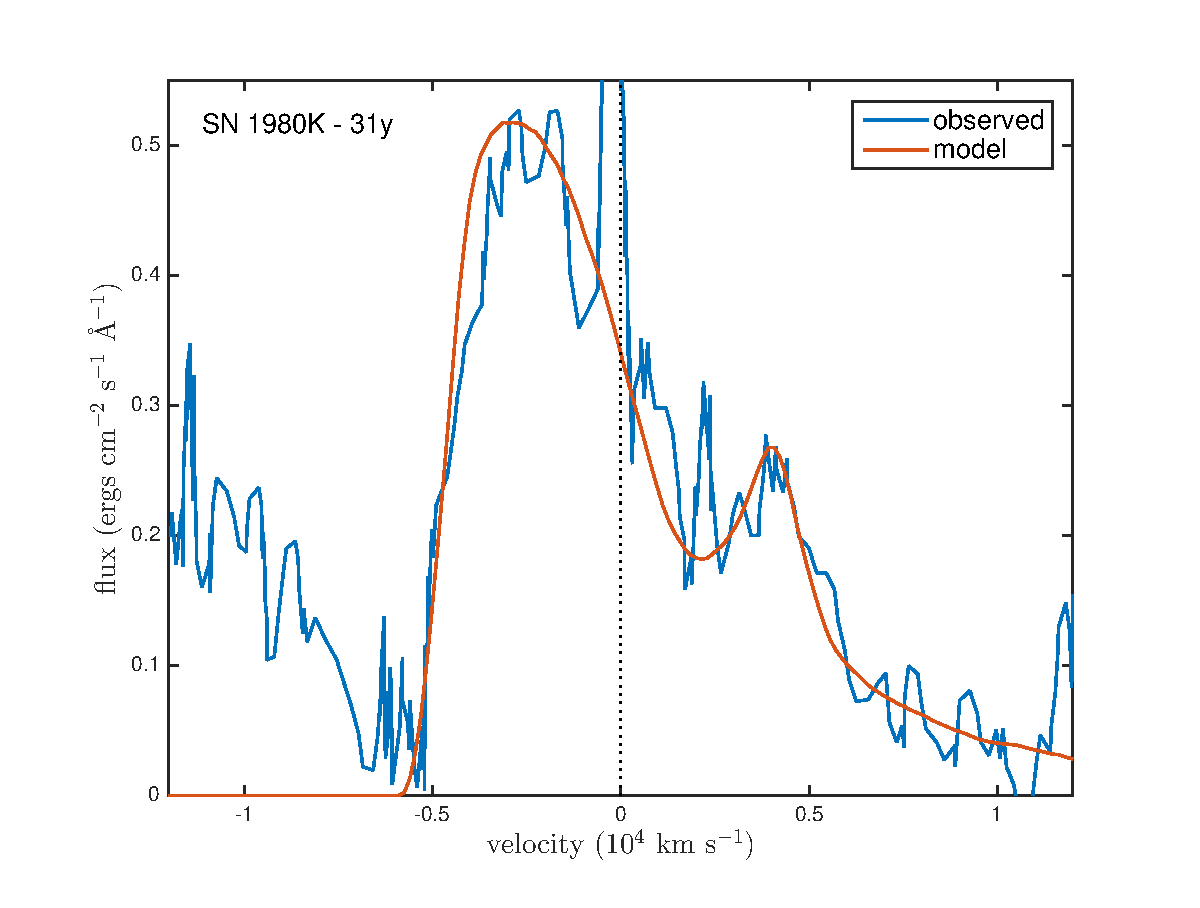
\includegraphics[scale=0.8,clip=true, trim=20 10 40 20]{chapters/chapter6/figs/80K/Ha_31y}

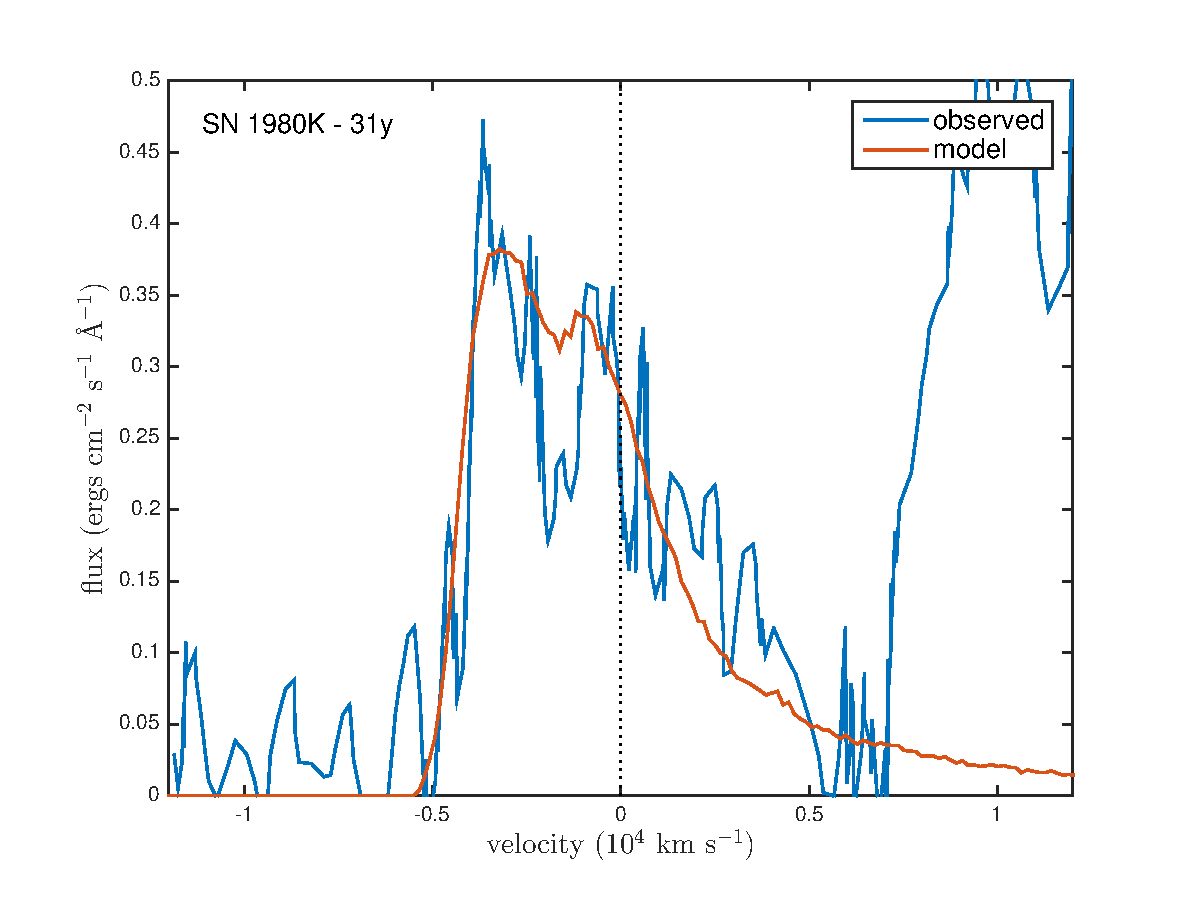
\includegraphics[scale=0.8,clip=true, trim=20 0 40 20]{chapters/chapter6/figs/80K/OI_31y}
\caption{Smooth fits to SN 1980K}
\label{80K_smooth}
\end{figure}

\begin{figure}
\centering
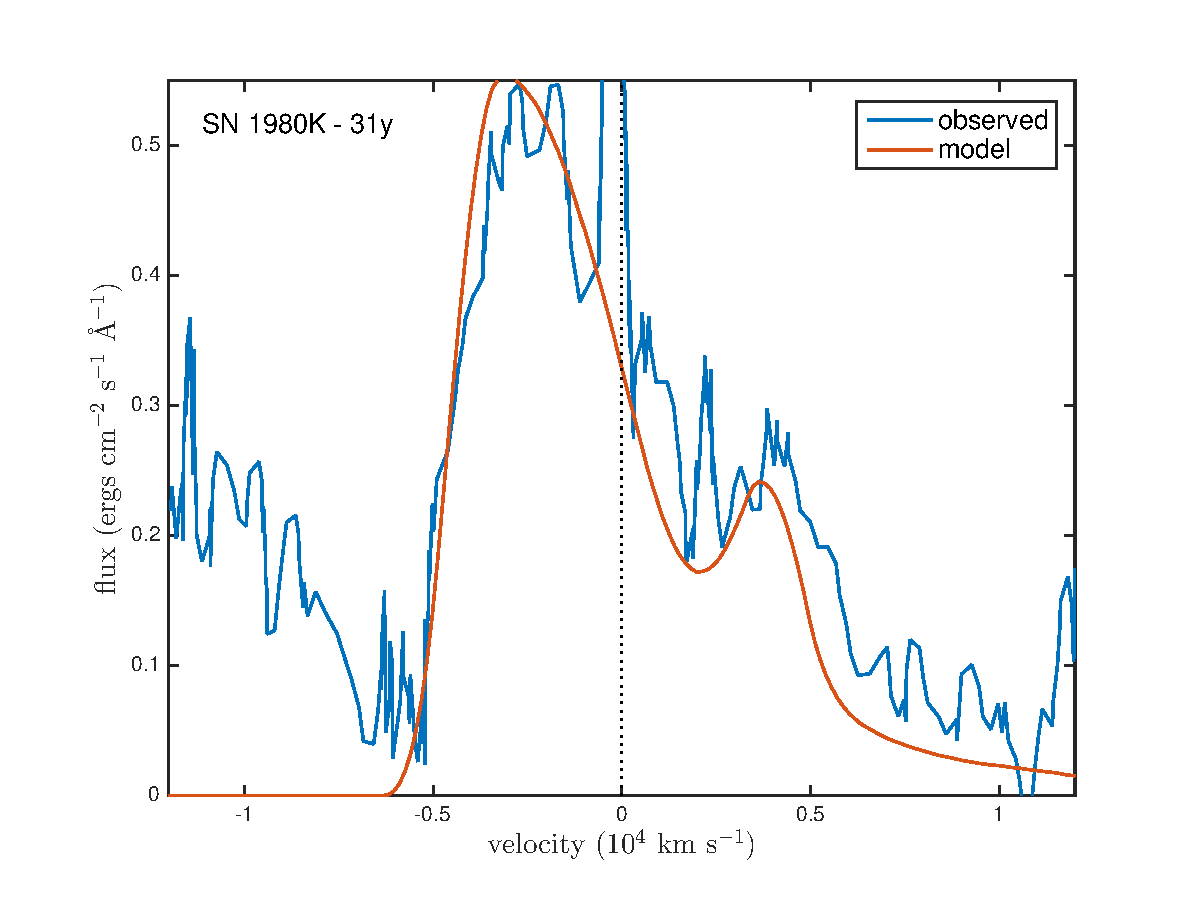
\includegraphics[scale=0.8,clip=true, trim=20 10 40 20]{chapters/chapter6/figs/80K/simultaneous/Ha_31y}

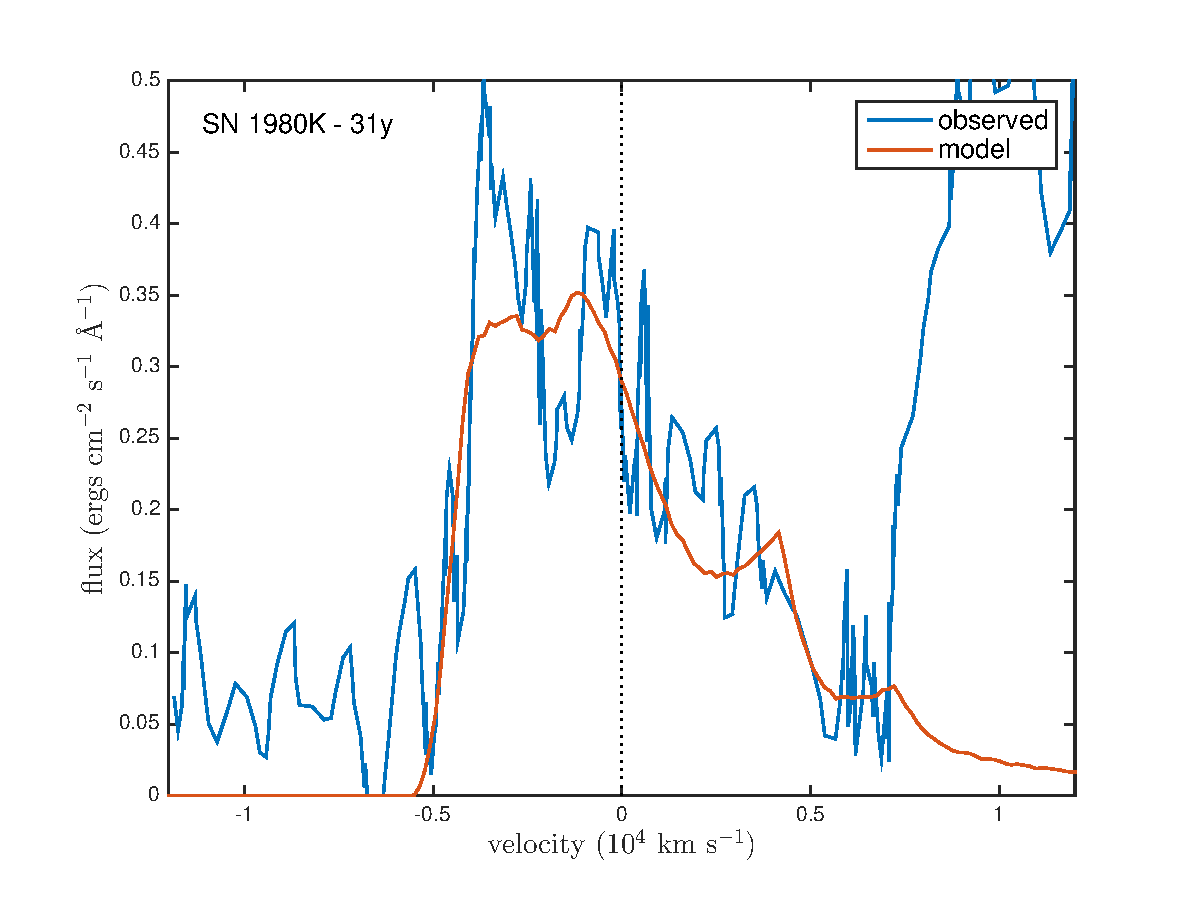
\includegraphics[scale=0.8,clip=true, trim=20 0 40 20]{chapters/chapter6/figs/80K/simultaneous/OI_31y}
\caption{Best fits to SN 1980K with unified dust distribution}
\label{80K_best}
\end{figure}

\section{SN 1993J}
\section{Cassiopeia A}
THE REST FOLLOW HERE. 


